%\newpage
\section{Ergebnisse und Berechnungen}
\label{sec:ergebnisse}

\subsection{Allgemeine Daten}
Aus den geometrischen Daten und den gemessenen Volumenströmen lassen sich die Daten der Tabellen \ref{tab:strom_reihe} und \ref{tab:strom_para} bestimmen. Diese sind relevant für weiterführende Berechnungen in den folgenden Abschnitten.

% Table generated by Excel2LaTeX from sheet 'Daten'
\begin{table}[h!]
	\renewcommand*{\arraystretch}{1.2}
	\centering
	\rowcolors{2}{gray!25}{white}
	\caption{Strömungsrelevante Größen der Reihenschaltung}
	\label{tab:strom_reihe}
	\resizebox{15cm}{!}{
		\begin{tabulary}{1.2\textwidth}{CCCCC}
			\hline
			\textbf{Strom}&\textbf{Fläche} $\left[\si{\sqm}\right]$&\textbf{hydr. Durchmesser} $\left[\si{\meter}\right]$&\textbf{Volumenstrom} $\left[\si{\cmt\per\second}\right]$&\textbf{Geschwindigkeit} $\left[\si{\meter\per\second}\right]$ \\
			\hline
			warm&\SI{7,85E-05}{}&\SI{0,010}{}&\SI{1,32E-04}{}&\SI{1,68}{}\\
			kalt	&\SI{6,83E-05}{}&\SI{0,003}{}&\SI{8,63E-05}{}&\SI{1,26}{}\\
			\hline			
		\end{tabulary}
	}
\end{table}%
\FloatBarrier

% Table generated by Excel2LaTeX from sheet 'Daten'
\begin{table}[h!]
	\renewcommand*{\arraystretch}{1.2}
	\centering
	\rowcolors{2}{gray!25}{white}
	\caption{Strömungsrelevante Größen der Parallelschaltung}
	\label{tab:strom_para}
	\resizebox{15cm}{!}{
		\begin{tabulary}{1.2\textwidth}{CCCCC}
			\hline
			\textbf{Strom}&\textbf{Fläche} $\left[\si{\sqm}\right]$&\textbf{hydr. Durchmesser} $\left[\si{\meter}\right]$&\textbf{Volumenstrom} $\left[\si{\cmt\per\second}\right]$&\textbf{Geschwindigkeit} $\left[\si{\meter\per\second}\right]$ \\
			\hline
			warm&\SI{7,85E-05}{}&\SI{0,010}{}&\SI{1,45E-04}{}&\SI{1,85}{}\\
			kalt	&\SI{6,83E-05}{}&\SI{0,003}{}&\SI{1,45E-04}{}&\SI{2,12}{}\\
			\hline			
		\end{tabulary}
	}
\end{table}%
\FloatBarrier

\subsection{Messdaten und Temperaturprofile}
Zunächst werden allgemein die theoretischen Messdaten in den Tabellen \ref{tab:messung_reihe} und \ref{tab:messung_para} für die Reihen- und Parallelschaltung dargestellt.

\begin{table}[h!]
		\centering
	\rowcolors{2}{gray!25}{white}
	\caption{Temperatur- und Druckmesswerte für die Reihenschaltung}
	\resizebox{7cm}{!}{
	\begin{tabulary}{\textwidth}{L|C|C}
		\textbf{Messstelle} & \textbf{Temperatur} $\left[\si{\celsius}\right]$& \textbf{Druck} $\left[\si{\bar}\right]$\\
		\hline
		$T_{\alpha,\text{warm}}$ & 55,38 & 1,030\\
		$T_{\text{zw1},\text{warm}}$  & 46,58 & 0,690  \\
		$T_{\text{zw2},\text{warm}}$  & 46,56 & 0,500\\
		$T_{\omega,\text{warm}}$  & 32,73 & 0,215 \\
		\hline
		$T_{\alpha,\text{kalt}}$  & 16,10 & 2,300\\
		$T_{\text{zw2},\text{kalt}}$   & 36,71 & 0,900  \\
		$T_{\text{zw1},\text{kalt}}$   & 36,75 & 1,300   \\
		$T_{\omega,\text{kalt}}$ & 49,68 & 0,065 \\
	\end{tabulary}%
}
	\label{tab:messung_reihe}%
\end{table}%
\FloatBarrier
\,
\begin{table}[h!]
	\centering
	\rowcolors{2}{gray!25}{white}
	\caption{Temperatur- und Druckmesswerte für die Parallelschaltung}
	\resizebox{7cm}{!}{
	\begin{tabulary}{\textwidth}{L|C|C}
		\textbf{Messstelle} & \textbf{Temperatur} $\left[\si{\celsius}\right]$& \textbf{Druck} $\left[\si{\bar}\right]$\\
		\hline
		$T_{1,\alpha,\text{warm}}$ & 55,54 & 0,200\\
		$T_{1,\omega,\text{warm}}$  & 30,71 & 0,152  \\
		$T_{2, \alpha,\text{warm}}$  & 55,63 & 0,310\\
		$T_{2,\omega,\text{warm}}$  & 31,52 & 0,300 \\
		\hline
		$T_{1,\alpha,\text{kalt}}$ & 16,21 & 1,530\\
		$T_{1,\omega,\text{kalt}}$  & 38,41 & 0,400  \\
		$T_{2, \alpha,\text{kalt}}$  & 16,30 & 1,580\\
		$T_{2,\omega,\text{kalt}}$  & 39,83 & 0,507 \\
	\end{tabulary}%
	}
	\label{tab:messung_para}%
\end{table}%
\FloatBarrier

Die Verläufe der Temperaturen für die einzelnen Wärmetauscher ergibt, zeigt sich in Abbildung \ref{dia:temp_profil}.

\vspace*{-7mm}

\begin{figure}[h!]
	\begin{center}
		\resizebox{0.7\textwidth}{!}{
			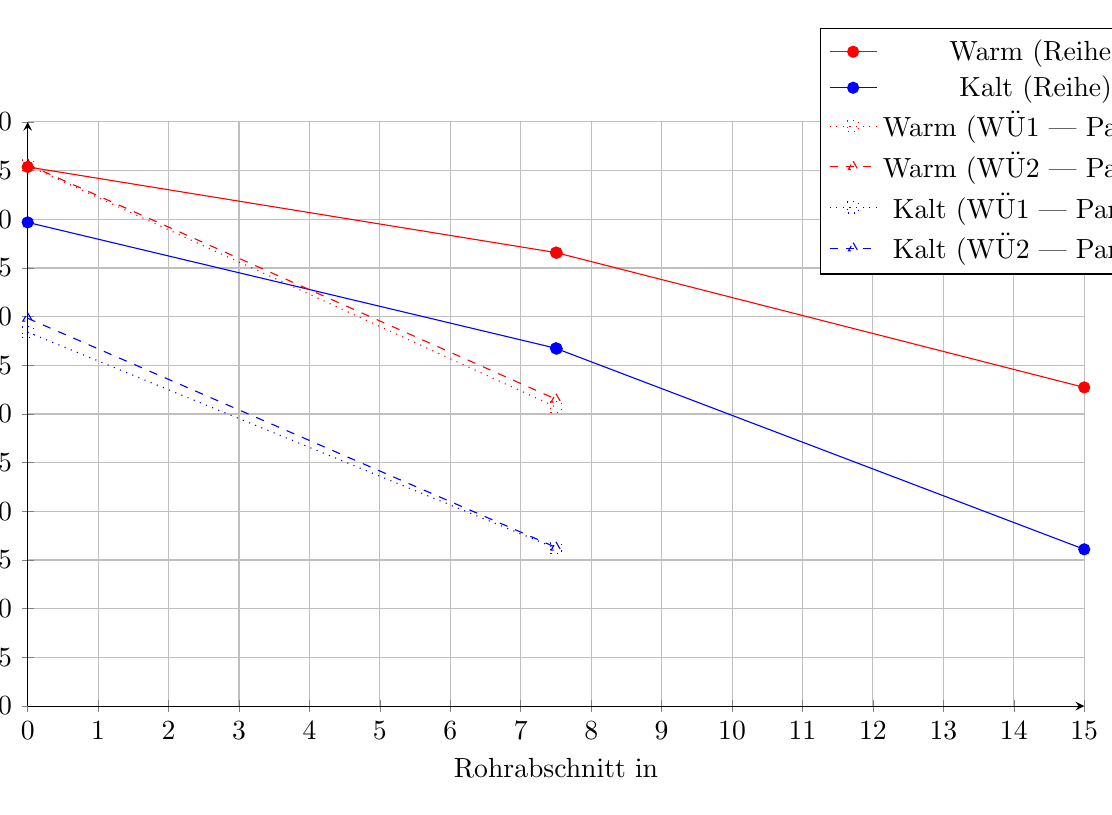
\begin{tikzpicture}[trim axis left, trim axis right]
			\begin{axis}[
			grid,
			axis lines = left,
			width = 15cm,
			height = 9cm,
			xmin = 0,
			xmax = 15,
			ymin = 0,
			ymax = 60,
			ytick = {0,5,...,60},
			xtick = {0,1,2,...,15},
			ylabel={Temperatur in \si{\celsius}},
			%y label style={at={(0,0.5)}},
			xlabel={Rohrabschnitt in \si{\meter}},
			legend style={at={(0.75,0.95)},anchor=west},
			%	y dir = reverse,
			]			
			%Warm Reihe
			\addplot [color=red, mark=*] coordinates{(0,55.38) (7.5,46.58) (7.51,46.56) (15, 32.73)};
			
			%Kalt Reihe
			\addplot [color=blue, mark=*] coordinates{(0,49.68) (7.5,36.75) (7.51,36.71) (15, 16.10)};
			
			%Warm Wü1
			\addplot [color=red, mark=square, dotted] coordinates{(0,55.54) (7.5, 30.71)};
			
			%Warm WÜ2
			\addplot [color=red, mark=triangle, dashed] coordinates{(0,55.63) (7.5, 31.52)};
			
			\addplot [color=blue, mark=square, dotted] coordinates{(0,38.41) (7.5, 16.21)};
			
			\addplot [color=blue, mark=triangle, dashed] coordinates{(0,39.83) (7.5, 16.30)};
			
			
			\legend{Warm (Reihe), Kalt (Reihe), Warm (WÜ1 | Parallel), Warm (WÜ2 | Parallel), Kalt (WÜ1 | Parallel), Kalt (WÜ2 | Parallel)}
			\end{axis}
			\end{tikzpicture}
		}
		\caption{Temperaturverläufe der Wärmetauscher}
		\label{dia:temp_profil}
	\end{center}
\end{figure}
\FloatBarrier

\subsection{Wärmeströme}
Um zu prüfen in welchem Maße der Wärmeübergang stattfindet, werden die Wärmeströme der verschiedenen Schaltungen untersucht. Dabei wird der gemessene Volumenstrom in der Berechnung mit einem Korrekturvolumenstrom angepasst. Daraus ergibt sich jeweils für die aufgenommene bzw. abgegebene Wärme ein korrigierter Volumenstrom. Genauere Beschreibungen hierzu finden sich in der Theorie unter Abschnitt \ref{sec:theorie}.\\
Zur Vereinfachung der Berechnungen wird eine konstante, spezifische Wärmekapazität angenommen. Die Dichten, welche für Berechnungen der Massenströme und den daraus resultierenden Wärmeströmen nötig sind, werden über die jeweils kälteste Temperatur des warmen bzw. kalten Stromes berechnet.\\
Die berechneten Werte finden sich in den Tabellen \ref{tab:warme_reihe} und \ref{tab:warme_para}.

% Table generated by Excel2LaTeX from sheet 'GegenstromReihe neu'
\begin{table}[h!]
	\renewcommand*{\arraystretch}{1.2}
	\centering
	\rowcolors{2}{white}{gray!25}
	\caption{Berechnete Wärmeströme und Korrekturvolumenstrom für die Reihenschaltung}
	\resizebox{15cm}{!}{
	\begin{tabulary}{1.2\textwidth}{C|CC|C|CC|C}
		\hline
		\textbf{System} & $\boldsymbol{Q_{ab}} \, \left[\si{\kilo \watt}\right]$ & $\boldsymbol{Q_{auf}} \, \left[\si{\kilo \watt}\right]$& $\boldsymbol{\dot{V}_{korr}} \, \left[\si{\cmt \per \second}\right]$& $\boldsymbol{Q_{ab, korr}} \, \left[\si{\kilo \watt}\right]$&$\boldsymbol{Q_{auf, korr}} \, \left[\si{\kilo \watt}\right]$ & $\boldsymbol{\Delta Q_{korr}} \, \left[\si{\kilo \watt}\right]$\\
		\hline
		WÜ1   & 7,58  & 7,44  &\SI{ -9,70E-07 }{}& 7,53  & 7,53  & 0,00 \\
		WÜ2   & 4,83  & 4,67  & \SI{-1,71E-06}{} & 4,76  & 4,76  & 0,00 \\
		\hline
		Gesamt & 12,42 & 12,13 & \SI{-1,24E-06}{} & 12,30 & 12,30 & 0,00 \\
		\end{tabulary}%
	}
	\label{tab:warme_reihe}%
\end{table}%
\FloatBarrier

% Table generated by Excel2LaTeX from sheet 'GegenstromReihe neu'
\begin{table}[h!]
	\renewcommand*{\arraystretch}{1.2}
	\centering
	\rowcolors{2}{white}{gray!25}
	\caption{Berechnete Wärmeströme und Korrekturvolumenstrom für die Parallelschaltung}
	\resizebox{15cm}{!}{
		\begin{tabulary}{1.2\textwidth}{C|CC|C|CC|C}
			\hline
			\textbf{System} & $\boldsymbol{Q_{ab}} \, \left[\si{\kilo \watt}\right]$ & $\boldsymbol{Q_{auf}} \, \left[\si{\kilo \watt}\right]$& $\boldsymbol{\dot{V}_{korr}} \, \left[\si{\cmt \per \second}\right]$& $\boldsymbol{Q_{ab, korr}} \, \left[\si{\kilo \watt}\right]$&$\boldsymbol{Q_{auf, korr}} \, \left[\si{\kilo \watt}\right]$ & $\boldsymbol{\Delta Q_{korr}} \, \left[\si{\kilo \watt}\right]$\\
			\hline
			WÜ1   & 7,50  & 6,72  &\SI{ -8,00E-06 }{}& 7,09 & 7,09 & 0,00 \\
			WÜ2   & 7,28 & 7,12  & \SI{-1,64E-06}{} & 7,20  & 7,20  & 0,00 \\
			\hline
			Gesamt   & 14,78 & 13,84  & \SI{-9,64E-06}{} & 14,29  & 14,29  & 0,00 \\
			\hline
		\end{tabulary}%
	}
	\label{tab:warme_para}%
\end{table}%
\FloatBarrier
\newpage
\subsection{Leistungen und Wärmeübertragungsparameter}
Um nun die Effizienz der Anlage besser beschreiben zu können, wird der transportierte Wärmestrom in ein Verhältnis zur elektrischen Leistung einer Kreiselpumpe mit 80\% Wirkungsgrad gesetzt. Diese Kreiselpumpe fördert die jeweilige Flüssigkeit durch das System.\\
Über die dimensionslosen Kennzahlen $Re$, $Pr$ und $Nu$ lassen sich nun die Wärmeübertragungsparameter $\alpha $ und $U$ berechnen. Über diese Werte lässt sich der Wärmeübertragungsprozess unabhängig von der Geometrie miteinander vergleichen. Zur Vereinfachung der Rechnungen wird die Wärmeleitfähigkeit vom Stahlrohr mit \SI{15}{\watt\per\meter \per\kelvin} angenommen. Die Wärmeleitfähigkeit des Fluides, sowie die Viskosität werden jedoch als Funktion von der Temperatur eingerechnet.\\
Die Ergebnisse dieser Rechnungen finden sich in den Tabellen \ref{tab:leistung_reihe} und \ref{tab:leistung_para} wieder und lassen sich mithilfe der theoretischen Grundlagen nachvollziehen.
\begin{table}[h!]
	\centering
	%\rowcolors{3}{gray!25}{white}{gray!10}
	\caption{Berechnete Leistungen, dimensionslose Kennzahlen und \linebreak Wärmeübertragungsparameter der Reihenschaltung}
	\resizebox{15cm}{!}{
	\begin{tabulary}{1.55\textwidth}{L|C|CCC||CCC|CC}
		\hline
		\textbf{System} & $\boldsymbol{\Delta p} \, \left[\si{\bar}\right]$ & $\boldsymbol{P_{Pumpe}} \, \left[\si{\kilo \watt}\right]$ &  $\boldsymbol{P_{Elektrisch}} \, \left[\si{\kilo \watt}\right]$& $\boldsymbol{Q/P_{Elektrisch}}$ & \textbf{Re} & \textbf{Pr}& \textbf{Nu} & $\boldsymbol{\alpha}  \, \left[\si{\kilo \watt \per \sqm \per \kelvin}\right]$ & $\boldsymbol{U} \, \left[\si{\watt \per \meter\per \kelvin}\right]$ \\
		\hline
		WÜ1 warm & 0,29  & \SI{3,76E-03}{} & \SI{4,70E-03}{}3 & 1602  & \SI{2,20E+04}{} & 5,13  & \SI{131,9}{} & 8,14  & \multirow{2}{*}{31,13}  \\
		WÜ1 kalt & 20,61 &\SI{ 1,78E-01 }{}&\SI{ 2,22E-01}{} & 34    &\SI{ 3,41E+03}{} & 7,87  & \SI{35,2 }{}& 6,93  &  \\
		\hline
		WÜ2 warm & 0,35  & \SI{4,66E-03 }{}& \SI{5,83E-03 }{}& 817   & \SI{2,87E+04}{} & 3,80  & \SI{144,5}{} & 9,20  & \multirow{2}{*}{34,98} \\
		WÜ2 kalt & 12,93 & \SI{1,12E-01}{} &\SI{ 1,40E-01 }{}& 34    & \SI{5,39E+03}{} & 4,68  & \SI{41,2}{} & 8,57  &  \\
		\hline
		Gesamt warm & 0,82  & \multirow{2}{*}{\SI{3,00E-02
			}{}}&  \multirow{2}{*}{\SI{3,76E-02}{}} & \multirow{2}{*}{328}   & -&- & -& - & -\\
		Gesamt kalt & 2,24  & & &    & -&- & -& - & -\\
		\hline
	\end{tabulary}%
}
	\label{tab:leistung_reihe}
\end{table}%
\vspace*{-5mm}
\begin{table}[h!]
	\centering
%	\rowcolors{2}{gray!25}{white}
	\caption{Berechnete Leistungen, dimensionslose Kennzahlen und \linebreak Wärmeübertragungsparameter der Parallelschaltung}
	\resizebox{15cm}{!}{
		\begin{tabulary}{1.55\textwidth}{L|C|CCC||CCC|CC}
			\hline
			\textbf{System} & $\boldsymbol{\Delta p} \, \left[\si{\bar}\right]$ & $\boldsymbol{P_{Pumpe}} \, \left[\si{\kilo \watt}\right]$ &  $\boldsymbol{P_{Elektrisch}} \, \left[\si{\kilo \watt}\right]$& $\boldsymbol{Q/P_{Elektrisch}}$ & \textbf{Re} & \textbf{Pr}& \textbf{Nu} & $\boldsymbol{\alpha}  \, \left[\si{\kilo \watt \per \sqm \per \kelvin}\right]$ & $\boldsymbol{U} \, \left[\si{\watt \per \meter\per \kelvin}\right]$ \\
			\hline
			WÜ1 warm & 0,06 & \SI{4,21E-04}{} & \SI{5,27E-04}{}& 13464  & \SI{1,16E+04}{} & 5,39  & \SI{80,62}{} & 4,96  & \multirow{2}{*}{23,97} \\
			WÜ1 kalt & 2,20 &\SI{ 1,60E-02 }{}&\SI{ 2,00E-02}{} & 354    &\SI{ 2,87E+03}{} & 7,83  & \SI{30,57}{}& 6,02  &  \\
			\hline
			WÜ2 warm & 0,01  & \SI{7,26E-05 }{}& \SI{9,08E-05 }{}& 79320   & \SI{1,18E+04}{} & 5,28  & \SI{81,10}{} & 4,99 & \multirow{2}{*}{24,08} \\
			WÜ2 kalt & 1,07 & \SI{7,79E-03}{} &\SI{ 9,74E-03 }{}& 739    & \SI{2,87E+03}{} & 7,83  & \SI{30,62}{} & 6,03 &  \\
			\hline
			Gesamt warm & 0,07  & \multirow{2}{*}{\SI{2,43E-02
				}{}}&  \multirow{2}{*}{\SI{3,04E-02}{}} & \multirow{2}{*}{471}   & -&- & -& - & -\\
			Gesamt kalt & 3,28 & & &    & -&- & -& - & -\\
			\hline
		\end{tabulary}%
}
	\label{tab:leistung_para}
\end{table}%

